% !TEX root = main.tex

\section{Graph-based inertial-kinematic odometry}

%We describe the inertial-kinematic odometry for legged robots, based on a graph model. 


%%%%%%%%%%%%%%%%%%%%%%%%%%%%%%%%%%%%%%%%%%%%%%%%%%%%%%%%%%%%

\subsection{Quaternion rotations}

We define the quaternion-by-vector product $\od$ so that
%
\begin{align}
\bfq\od\bfv \te \bfq\ot\bfv\ot\bfq^*
~,
\end{align}
%
where $\bfq^*$ denotes the dual quaternion of $\bfq$. 
The symbol $\ot$ stands for the product of quaternions and $\od$ corresponds to the quaternion-by-vector which performs a 3D rotation of an input vector $\bfv$. 
Notice that if $\bfR$ is the rotation matrix equivalent to the quaternion $\bfq$, then 
%
$\bfq\od\bfv = \bfR\,\bfv$. 
%
This straightforward equivalence
enables us to define all the forthcoming IMU pre-integration algebra in a way that allows a direct transcription between the $S^3$  and $SO(3)$ spaces of representation.

%%%%%%%%%%%%%%%%%%%%%%%%%%%%%%%%%%%%%%%%%%%%%%%%%%%%%%%%
\subsection{Graph-based iterative optimization}

In graph-based optimization, the problem is represented as a graph, where the nodes refer to the variables, and the edges, called factors, represent the geometrical constraints that link between variables produced by the measurements.
%
The state $\bfx$ is modeled as a multi-variate Gaussian distribution, and in our case it includes foot poses and velocities $(\bfp,\bfq,\bfv)$ and IMU biases $(\bfa_b,\bw_b)$ at selected keyframes along the trajectory (see \figRef{fig:factor_graph}).
%
For each factor, we can define an error or a residual $\bfr$ as the discrepancy between a measurement $\bfz$ and its expectation given the involved state variables,
%
\begin{equation}
    \bfr(\bfx) = h(\bfx) + \bfv - \bfz, \qquad \bfv \sim \mathcal \cN (0, \bfOmega\inv)\label{eq:error}
\end{equation}
%
being $h(\bfx)$ the sensor measurement model and $\bfOmega$ the information matrix of the measurement Gaussian noise $\bfv$.
Importantly, the functions $h(\bfx)$ and $\bfr(\bfx)$ are very sparse, since only a small handful of blocks of $\bfx$ are involved in each factor, which results in a loosely connected graph.
In case of variables defined on manifolds, such as quaternions or rotation matrices, we must rewrite~\eqref{eq:error} as \mbox{$\bfr(\bfx) = (h(\bfx) \oplus \bfv) \ominus \bfz$}.
%, with $\bfJ_k = \partial (h_k(\bfx)\ominus\bfz_k)/\partial \Delta \bfx$. 
The $\oplus$ and $\ominus$ symbols correspond to the addition and subtraction operators on the manifold
%, as required for certain state blocks intervening in the factor 
(see \eg~Eq.~\eqRef{equ:imu_residual} in \secRef{sec:imu}, or Eq.~\eqsRef{equ:plus_q}{equ:minus_R} in \appRef{sec:derivatives_SO3}).

The maximum a posteriori estimation is obtained by iteratively minimizing the Mahalanobis squared norm of all linearized errors
%
\begin{align}
  \Delta \bfx^* &= \argmin_{\Delta \bfx} \sum_k \norm{ \bfr_k(\breve\bfx) + \bfJ_k \Delta \bfx }_{\bfOmega_k^{-1}}^2 \label{eq:LeastSquares}
\end{align}
%
being $\breve\bfx$ the state estimate at the current iteration, and $\bfJ_k$ the Jacobian of the $k$-th residual $\bfr_k(\bfx)$ (with \mbox{$\bfJ_k = \partial (h_k(\bfx)\ominus\bfz_k)/\partial \Delta \bfx$} in the case of variables lying on a manifold) and $\bfOmega_k$ is the information matrix of the $k$-th measurement.
%
Current methods use the Cholesky~\cite{Kummerle_icra11,ila_ijrr17} or the QR~\cite{Dellaert_ijrr06,Kaess_ijrr11} matrix factorizations to solve for $\Delta\bfx^*$, which is then used to update the current state estimate. 
The process is iterated until convergence.
%
Incremental methods~\cite{ila_ijrr17,Kaess_ijrr11} update the problem directly on the factorized matrices, obtaining important speed-ups.


%%%%%%%%%%%%%%%%%%%%%%%%%%%%%%%%%%%%%%%%%%%%%%%%%%%%%%%%%

%Estimation is realized with a tool in ongoing development \textbf{(cite WOLF ?)} and using Google Ceres non-linear least squares optimizer. This optimization is run on data given by the front-end part of the framework,
%which aim is to formalize the problem according to the graph-based model for aforementioned reasons. This representation, illustrated in \figRef{fig:factor_graph}, 
%gives a human-readable way to easily visualize optimized states (circles) linked to constraining information during the optimization process (factors drawn as squares). Constraints are set by the front-end process using measurements from sensors.
%Thus, it is possible to constrain states with several factors provided by different sensors leading to a fusion. Factor play a key role since they are used on top of previous states to predict next ones and compute the error with the current states.
%The optimal states are computed so that the overall residual is minimized in a least squares meaning.


\begin{figure}[tb]
\centering
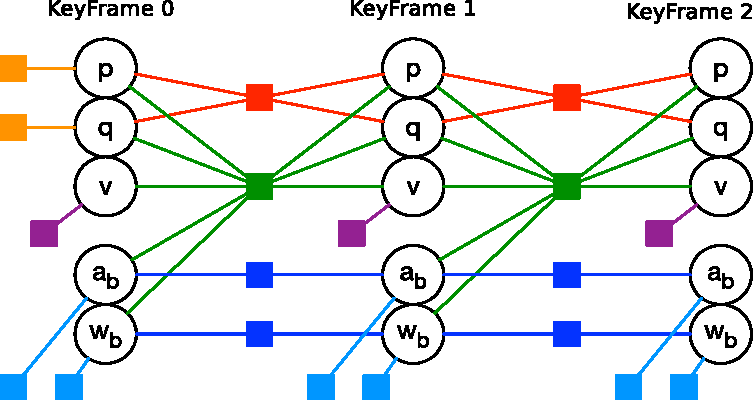
\includegraphics[scale=0.65]{figures/graph_exploded}
\caption{
%{\bf Top}: 
Detailed factor graph for the initial keyframe and two steps. 
\emph{Circles}: state blocks for position ($\bfp$), orientation quaternion ($\bfq$), velocity ($\bfv$), accelerometer bias ($\bfa_b$), gyrometer bias ($\bw_b$). 
\emph{Orange}: initial pose factor. 
\emph{Red}: kinematic factor (deduced from additional sensors). 
\emph{Purple}: zero-velocity factor. 
\emph{Green}: IMU's delta pre-integration factor. 
\emph{Blue}: bias drift factor. 
\emph{Cyan}: bias absolute factor. 
%{\bf Bottom}: Equivalent factor graph exhibiting one aggregate state block $\bfx=(\bfp,\bfq,\bfv,\bfa_b,\bw_b)$ for each key-frame. All factors are affecting exactly the same variables as in the Top graph.
}
\label{fig:factor_graph}
\end{figure}



%%%%%%%%%%%%%%%%%%%%%%%%%%%%%%%%%%%%%%%%%%%%%%%%%%%%%
%\subsection{Graph-based inertial-kinetic odometry}

\subsection{Keyframe variables}

During a biped walk, we take profit of certain situations where precise and reliable assumptions can be made. For example, the  foot velocity is null during its support phase. At these selected instants, we create the keyframes that will produce a chain of states. These states are linked by the measurements, forming our factor graph (\figRef{fig:factor_graph}). Each keyframe $\bff_i$ contains the following state blocks: the foot's position, velocity and orientation data, plus the IMU's accelerometer and gyrometer biases,
%
\begin{align}
\bff_i = \begin{bmatrix}
\bfp_i & \bfv_i & \bfq_i & \bfa_{b,i} & \bw_{b,i}
\end{bmatrix}\tr
~.
\end{align}
%


%%%%%%%%%%%%%%%%%%%%%%%%%%%%%%%%%%%%%%%%%%%%%%%%%%%%%
\subsection{Description of factors}

The types of factor considered in our graph are illustrated in \figRef{fig:factor_graph}. 
Each factor $k$ requires its own information matrix~$\bfOmega_k$, and its residual function $\bfr_k(\bfx)$. These residual functions are detailed hereafter.

\subsubsection{Absolute factors}

These include initial position and orientation (orange in the figure), zero velocity (purple), and bias magnitude (cyan). Each residual depends on a single state block, which is compared against a reference $\bfz_k$,
%
\begin{align}
\bfr_k(\bfphi_i) = \bfphi_i - \bfz_k
\end{align}
%
where $\bfphi_i$ is one among $\{\bfp_i,\bfv_i,\bfa_{b,i},\bw_{b,i}\}$. 
For the quaternion we implement the residual using the operator $\ominus$ on the sphere of dimension $3$ manifold, denoted $S^3$ (see \eqRef{equ:minus_q} in \appRef{sec:derivatives_SO3} for further details),
%
\begin{align}
\bfr_k(\bfq_i) = \bfq_i\ominus\bfz_k = \Log(\bfz_k^*\ot\bfq_i)
\end{align}
%

\subsubsection{Bias drift factors (blue)}

These are relative factors that allow the bias estimates to drift with time at a controlled rate. Each bias drift residual depends on two state blocks, namely
%
\begin{align}
\begin{split}
\bfr(\bfa_{b,i}, \bfa_{b,j}) &= \bfa_{b,j} - \bfa_{b,i} 
\\
\bfr(\bw_{b,i} , \bw_{b,j})  &= \bw_{b,j}  - \bw_{b,i}
\end{split}
\end{align}

\subsubsection{Complementary factors (red)}

These relate position and orientation between two consecutive steps as it can be provided by other sensors than IMU or methods using human walking specificities,
%
\begin{align}
\bfr(\bfp_i,\bfq_i,\bfp_j,\bfq_j) = \begin{bmatrix}
\bfq_i^*\od(\bfp_j-\bfp_i) - \bfy_k \\
\Log(\bfz_k^*\ot\bfq_i^*\ot\bfq_j)
\end{bmatrix}
\end{align}
%
where $\bfy_k$ and $\bfz_k$ are respectively the relative position and quaternion measurements.

\subsubsection{IMU pre-integrated factors (green)}

These factors are by far the most complex ones and are described in details in the next section.
